
\documentclass[conference]{IEEEtran}
\IEEEoverridecommandlockouts
\usepackage{cite}
\usepackage{amsmath,amssymb,amsfonts}
\usepackage{algorithm}
\usepackage{algpseudocode}
\usepackage{graphicx}
\usepackage{booktabs}
\usepackage{multirow}
\usepackage{xcolor}
\usepackage{tikz}
\usetikzlibrary{arrows.meta,positioning,fit,shapes.geometric}
\usepackage{url}
\graphicspath{{figures/}}

\newcommand{\NTotal}{41,794}
\newcommand{\NTrain}{29,255}
\newcommand{\NVal}{6,269}
\newcommand{\NTest}{6,270}
\newcommand{\IGk}{5,000}
\newcommand{\NFeat}{5,009}
\newcommand{\MetaLearner}{Logistic Regression}
\newcommand{\StackAcc}{99.54}
\newcommand{\StackFone}{0.9956}
\newcommand{\StackFPR}{0.47}
\newcommand{\StackFN}{15}
\newcommand{\StackFP}{14}
\newcommand{\LRAcc}{99.51}
\newcommand{\HybAcc}{99.51}
\newcommand{\HybFone}{0.9953}
\newcommand{\HybRec}{0.9955}
\newcommand{\HybFPR}{0.54}
\newcommand{\HybFN}{15}
\newcommand{\HybFP}{16}
\newcommand{\CLKAcc}{98.25}
\newcommand{\CLKk}{400}
\newcommand{\CLKtau}{1.0}
\newcommand{\StageTwoFlips}{2}
\newcommand{\StageTwoCorrect}{0}
\newcommand{\StageOneMissed}{15}
\newcommand{\StackTrainTime}{72.6}
\newcommand{\StackTestTime}{5.4}
\newcommand{\XCLStackFone}{0.3647}
\newcommand{\XCLStackRec}{0.2626}
\newcommand{\XCLStackAcc}{85.37}
\newcommand{\XCLHybFone}{0.2898}
\newcommand{\XCLHybRec}{0.2670}
\newcommand{\XCLHybAcc}{79.08}
\newcommand{\XCLCLKFone}{0.2383}
\newcommand{\XCLCLKRec}{0.5011}
\newcommand{\XCLCLKAcc}{48.78}
\newcommand{\XCLNtest}{2,858}
\newcommand{\XCLNtrain}{27,254}
\newcommand{\XLCStackFone}{0.7920}
\newcommand{\XLCStackRec}{0.8712}
\newcommand{\XLCStackAcc}{74.53}
\newcommand{\XLCHybFone}{0.7941}
\newcommand{\XLCHybRec}{0.8755}
\newcommand{\XLCHybAcc}{74.73}
\newcommand{\XLCCLKFone}{0.8367}
\newcommand{\XLCCLKRec}{0.8502}
\newcommand{\XLCCLKAcc}{81.53}
\newcommand{\XLCNtest}{5,842}
\newcommand{\XLCNtrain}{2,001}
\newcommand{\LingMajority}{84.01}
\newcommand{\HaveGemini}{0}
\newcommand{\TauEightRec}{0.9988}
\newcommand{\TauEightFPR}{1.15}
\newcommand{\TauEightFN}{4}


\begin{document}

\title{HMS-PED: A Hybrid Multi-Stage Phishing Email Detector Adapting the HMS-IDS Framework, with Large Language Model Escalation in a Browser Extension}

% ---------------- EDIT: your team's details ----------------
\author{
\IEEEauthorblockN{Sameer Hembram (S24CSEU0453)}
\IEEEauthorblockA{\textit{Dept. of Computer Science and Engineering} \\
\textit{Bennett University}\\
Greater Noida, India}
\and
\IEEEauthorblockN{Ayushmaan Kumar (S24CSEU2784)}
\IEEEauthorblockA{\textit{Dept. of Computer Science and Engineering} \\
\textit{Bennett University}\\
Greater Noida, India}
}

\maketitle

\begin{abstract}
Phishing email remains the most common entry point for cyber attacks. Detectors built on large language models (LLMs) can explain their decisions in plain language, but they are slow, costly per message, send email content to a third party, and are rarely evaluated on more than a few hundred emails. We adapt the Hybrid Multi-Stage Intrusion Detection System (HMS-IDS), originally proposed for zero-day attacks in industrial IoT networks, to phishing email detection and integrate it into an existing Gmail browser extension that previously relied on an LLM alone. Stage~1 is a stacking ensemble of Naive Bayes, Decision Tree, $k$-Nearest Neighbours and Logistic Regression over Information-Gain-selected text features and hand-crafted phishing indicators. Stage~2 is the HMS-IDS cluster-labelling $k$-means (CL-$k$-means) anomaly layer, which re-examines emails that Stage~1 considers legitimate. Stage~3 escalates uncertain emails to the Gemini LLM and produces a human-readable explanation. On a stratified 70/15/15 split of \NTotal{} de-duplicated emails from the public Ling and CEAS-2008 corpora, the stacking ensemble reaches \StackAcc\% accuracy (F1 \StackFone, false-positive rate \StackFPR\%). However, when the same pipeline is trained on one corpus and tested on the other, F1 falls to \XCLStackFone{} (CEAS$\rightarrow$Ling), and the CL-$k$-means layer does not recover it. This exposes a generalisation gap that in-distribution accuracy hides, and it motivates the LLM escalation stage. The code, data splits and results are released for reproducibility.
\end{abstract}

\begin{IEEEkeywords}
Phishing detection, ensemble learning, stacking, $k$-means, large language models, browser extension, email security
\end{IEEEkeywords}

% =====================================================================
\section{Introduction}
Phishing emails impersonate trusted senders to steal credentials or deliver malware, and they remain a leading initial-access vector. Classical defences combine blocklists with supervised classifiers trained on labelled emails \cite{fette2007learning,abunimeh2007comparison}. More recently, LLMs have been used as zero-shot phishing detectors that also explain their verdicts \cite{koide2024chatspamdetector,heiding2024devising}.

Our base paper, Pham \emph{et al.} \cite{pham2025demo}, presented an LLM-based browser extension for phishing detection. This project builds on its open-source implementation: a Chrome extension that reads the open Gmail message and uses Google's Gemini model to decide whether it is phishing \cite{cmpe209repo}. Whilst the design is attractive as all results have an explanation, there are 4 problems: each scan makes an API call over the network, the whole email is sent to a third party, the model can be tricked by text hidden in the email \cite{greshake2023indirect}, and its published evaluation used only 200 CEAS and 100 SpamAssassin emails \cite{pham2025demo}.

Our reference framework, HMS-IDS \cite{saurabh2025hmsids}, faced an analogous problem in network intrusion detection. Supervised models detect \emph{known} attacks well but miss \emph{zero-day} ones. HMS-IDS addresses this with two tiers: a stacking ensemble of four simple learners, followed by an unsupervised cluster-labelling $k$-means layer to review traffic that was deemed benign by the stacking ensemble. We have used this framework and extended it by adding an LLM layer. 

The contributions of this work are:
\begin{enumerate}
\item \textbf{HMS-PED}, an adaptation of HMS-IDS to phishing email detection. It uses Information-Gain feature selection, a stacking ensemble of NB, DT, KNN and LR, and the CL-$k$-means anomaly layer with a cluster-purity threshold $\tau$, extended with an LLM escalation stage.
\item A reproducible evaluation on \NTotal{} emails with a fixed stratified train/validation/test split. All hyper-parameters are chosen on the validation set only.
\item An \emph{unseen-corpus} protocol, the email analogue of zero-day evaluation, which shows that near-perfect in-distribution scores do not transfer across corpora.
\item Integration of the full pipeline into the original browser extension, including a fix for its email-capture defect.
\end{enumerate}

% =====================================================================
\section{Related Work}
\subsection{Machine-learning phishing and spam detection}
Fette \emph{et al.} \cite{fette2007learning} showed that a small set of structural features (e.g., number of links, IP-based URLs, HTML content) lets a classifier detect phishing with high accuracy. Abu-Nimeh \emph{et al.} \cite{abunimeh2007comparison} compared logistic regression, trees, random forests, SVMs and neural networks on the same task and found trade-offs between false positives and false negatives across the models. Androutsopoulos \emph{et al.} \cite{androutsopoulos2000lingspam} introduced the Ling-Spam corpus used here and evaluated Naive Bayes filtering on it. Champa \emph{et al.} \cite{champa2024curated,champa2023zenodo} curated several public corpora, including Ling and CEAS-2008, into a common format, which we use directly.

\subsection{LLM-based detection}
ChatSpamDetector \cite{koide2024chatspamdetector} prompts GPT-family models to classify emails and justify the decision. Heiding \emph{et al.} \cite{heiding2024devising} studied LLMs both for writing and for detecting phishing emails and reported LLM-based detection as promising. LLM detectors also inherit the risks of LLM-integrated applications, notably indirect prompt injection \cite{greshake2023indirect}. Pham \emph{et al.} \cite{pham2025demo} demonstrated an LLM-based browser extension that classifies the open email and explains its verdict; it is the base paper of this work. Beyond email, Rahman \emph{et al.} \cite{rahman2025grid} examine LLMs for the cybersecurity of power distribution grids, a setting close to the industrial-IoT domain of our reference framework, where reliability of and trust in model output are similar concerns to ours.

\subsection{The reference framework: HMS-IDS}
Saurabh \emph{et al.} \cite{saurabh2025hmsids} proposed HMS-IDS for industrial IoT networks. After pre-processing and Information-Gain feature selection, a stacking ensemble of Decision Tree, KNN, Logistic Regression and Naive Bayes, with the best base learner as meta-learner, detects known attacks. Samples the ensemble labels \emph{normal} go to a CL-$k$-means model: clusters are labelled by majority class, and a test sample inherits the label of its nearest cluster together with a confidence equal to the cluster's purity. HMS-IDS reports 99.49\% accuracy on CIC-ToN-IoT. This work maintains this two-level hierarchy. However, we change the domain of data used (email text instead of network flows), how features are extracted, and what is considered as `unknown' threats. 

% =====================================================================
\section{Datasets}
We use the Ling and CEAS-2008 corpora as distributed by Champa \emph{et al.} \cite{champa2023zenodo}, the same files shipped with the original extension \cite{cmpe209repo}. Label 1 denotes a phishing/malicious email and 0 a legitimate one. Subjects and bodies are whitespace-normalised, bodies are truncated to 5,000 characters, empty emails are removed, and exact duplicates of (subject, body) are dropped. This leaves \NTotal{} emails.

The data are split 70/15/15 into training, validation and test sets, stratified jointly on label and source corpus, with a fixed random seed (Table~\ref{tab:data}). The validation split is used for every tuning decision, and the test split is used once for the final numbers. This differs from HMS-IDS, which reports 10-fold cross-validation on a 70/30 split; we also report 5-fold cross-validation accuracy on the training split for comparison.

\begin{table}[t]
\centering
\caption{Data splits (stratified on label and corpus)}
\label{tab:data}
\begin{tabular}{lrrr}
\toprule
Split & Emails & Phishing & Legitimate\\
\midrule
Train & 29,255 & 15,491 & 13,764\\
Validation & 6,269 & 3,320 & 2,949\\
Test & 6,270 & 3,320 & 2,950\\
\midrule
Total & 41,794 & 22,131 & 19,663\\
\bottomrule
\end{tabular}

\end{table}

% =====================================================================
\section{Proposed Methodology}
\subsection{Architecture}
Fig.~\ref{fig:arch} shows the pipeline. A browser extension extracts details of the email senders, subject line and email body. The information is then sent to a local Flask service. Stage 1 determines the likelihood the email is a phishing email. If the email is determined to be legitimate in stage 1, it is passed to stage 2. From here, if it is found to still be legitimate but is unclear, it will be passed to stage 3 where the LLM can determine the outcome. The LLM will also create the explanation that will be shown to the user.

\begin{figure}[t]
\centering
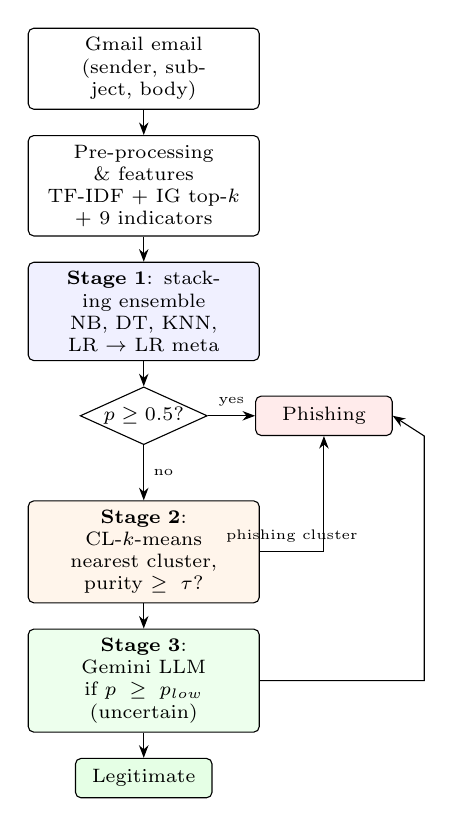
\begin{tikzpicture}[
  node distance=3.2mm and 4mm,
  box/.style={draw, rounded corners=2pt, align=center, font=\scriptsize, minimum height=6mm, text width=27mm, fill=white},
  dec/.style={draw, diamond, aspect=2.2, align=center, font=\scriptsize, inner sep=0.5pt, fill=white},
  res/.style={draw, rounded corners=2pt, align=center, font=\scriptsize, minimum height=5mm, text width=15mm},
  arr/.style={-{Stealth[length=1.6mm]}, thin}]
\node[box] (in) {Gmail email\\(sender, subject, body)};
\node[box, below=of in] (pre) {Pre-processing \& features\\TF-IDF + IG top-$k$ + 9 indicators};
\node[box, below=of pre, fill=blue!6] (s1) {\textbf{Stage 1}: stacking ensemble\\NB, DT, KNN, LR $\rightarrow$ LR meta};
\node[dec, below=of s1] (d1) {$p \ge 0.5$?};
\node[box, below=7mm of d1, fill=orange!8] (s2) {\textbf{Stage 2}: CL-$k$-means\\nearest cluster, purity $\ge\tau$?};
\node[box, below=of s2, fill=green!7] (s3) {\textbf{Stage 3}: Gemini LLM\\if $p\ge p_{low}$ (uncertain)};
\node[res, right=6mm of d1, fill=red!8] (ph) {Phishing};
\node[res, below=of s3, fill=green!10] (lg) {Legitimate};
\draw[arr] (in) -- (pre);
\draw[arr] (pre) -- (s1);
\draw[arr] (s1) -- (d1);
\draw[arr] (d1) -- node[above, font=\tiny] {yes} (ph);
\draw[arr] (d1) -- node[right, font=\tiny] {no} (s2);
\draw[arr] (s2.east) -| node[pos=0.25, above, font=\tiny] {phishing cluster} (ph.south);
\draw[arr] (s2) -- (s3);
\draw[arr] (s3.east) -| ([xshift=4mm]ph.south east) -- (ph.east);
\draw[arr] (s3) -- (lg);
\end{tikzpicture}
\caption{HMS-PED pipeline. Stages 1--2 follow HMS-IDS \cite{saurabh2025hmsids}; Stage 3 and the explanation reuse the LLM prompt of the original extension \cite{cmpe209repo}.}
\label{fig:arch}
\end{figure}

\subsection{Feature engineering}
Subject and body are concatenated and represented by TF-IDF weights \cite{salton1988term} over word unigrams and bigrams (minimum document frequency 3, at most 30,000 terms, sublinear term frequency). As in HMS-IDS, features are ranked by Information Gain (IG) \cite{yang1997comparative}. For target $Y$ and the binary presence $X_t$ of term $t$,
\begin{equation}
IG(Y;X_t) = H(Y) - \sum_{v\in\{0,1\}} P(X_t{=}v)\,H(Y\mid X_t{=}v),
\end{equation}
where $H$ is Shannon entropy. The number of retained terms $k\in\{1000,3000,5000\}$ is chosen on the validation split, giving $k=\IGk$. Nine hand-crafted indicators are appended, scaled to $[0,1]$: number of URLs, URL presence, URLs with raw IP addresses, exclamation marks, upper-case ratio of body and subject, currency symbols, log body length, and occurrences of urgency or credential words (e.g., \emph{verify}, \emph{suspend}, \emph{password}). The final vector has \NFeat{} dimensions. Fig.~\ref{fig:ig} lists the highest-IG terms. They are not phishing cues but markers of the legitimate mailing-list discussions in CEAS (\emph{wrote}, \emph{re}, \emph{mailing list}) and common function words. Most of the discriminative signal therefore comes from what legitimate email in this corpus looks like, which anticipates the generalisation problem in Section~\ref{sec:cross}.

\begin{figure}[t]
\centering
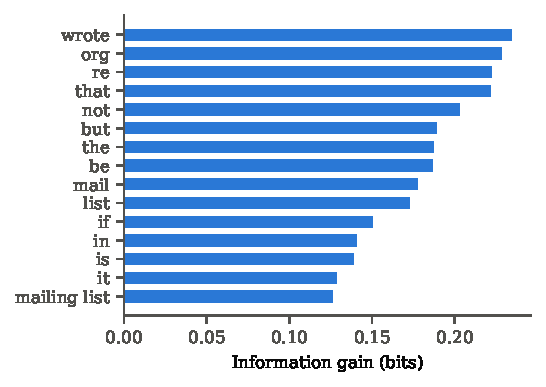
\includegraphics[width=0.85\columnwidth]{fig_ig_terms}
\caption{Top-15 terms by Information Gain on the training split.}
\label{fig:ig}
\end{figure}

\subsection{Stage 1: stacking ensemble}
Following HMS-IDS, four base learners are trained: multinomial Naive Bayes, Decision Tree, KNN (cosine distance) and Logistic Regression. Each one's hyper-parameters (smoothing $\alpha$, maximum depth, number of neighbours, inverse regularisation $C$) are chosen on the validation split. The tuned learners are combined by stacking \cite{wolpert1992stacked}. Out-of-fold class probabilities from 5-fold cross-validation train a meta-learner. As in HMS-IDS, the meta-learner is the algorithm of the best base learner on validation, which here is \MetaLearner. All models use scikit-learn \cite{pedregosa2011sklearn}.

\subsection{Stage 2: CL-$k$-means anomaly layer}
Emails are embedded with truncated SVD (100 components) of the Stage~1 features and L2-normalised. Mini-batch $k$-means \cite{sculley2010webscale} partitions the training emails into $k$ clusters. Each cluster $C_j$ receives the majority label $M_j$ and the HMS-IDS confidence (purity)
\begin{equation}
\mathrm{conf}(C_j)=\frac{|\{x\in C_j : y(x)=M_j\}|}{|C_j|}.
\end{equation}
An email that Stage~1 labels legitimate is re-labelled phishing if its nearest cluster has $M_j=1$ and $\mathrm{conf}(C_j)\ge\tau$. Here we add the threshold $\tau$ to the HMS-IDS rule. The cluster count $k\in\{50,100,200,400\}$ is chosen by the stand-alone validation F1 of CL-$k$-means ($k=\CLKk$), and $\tau$ by the validation F1 of the full hybrid ($\tau=\CLKtau$).

\subsection{Stage 3: LLM escalation and explanation}
Emails that remain legitimate but have a Stage~1 phishing probability $p\ge p_{low}$ (default 0.05) are sent to Gemini \cite{gemini2023} with the zero-shot prompt of the original extension \cite{cmpe209repo}. The prompt asks for a JSON answer with an \texttt{is\_phishing} flag and a short explanation. A phishing verdict from the LLM overrides the legitimate label. Confident decisions never wait for an API call, and only uncertain emails leave the user's machine for classification.

\subsection{Browser-extension integration}\label{sec:ext}
Rather than requesting the open email via an event listener that listens for changes to the Gmail page, we request it directly from the content script when the popup opens. We have created a new endpoint at \texttt{/api/hybrid-scan}, which runs stages 1-3 and returns the verdict, the chance of phishing and the stage at which the verdict was decided. The original LLM only endpoint has been retained.

\subsection{Evaluation metrics}
We report accuracy, precision, recall, F1, and the false-positive rate $\mathrm{FPR}=FP/(FP+TN)$, with phishing as the positive class. The FPR matters because a flagged legitimate email erodes user trust.

% =====================================================================
\section{Results and Discussion}
\subsection{In-distribution performance}
Table~\ref{tab:main} and Fig.~\ref{fig:metrics} give test-split results. Logistic Regression is the strongest single learner (\LRAcc\% accuracy), and stacking improves it slightly to \StackAcc\% (F1 \StackFone). Stacking misses \StackFN{} phishing emails and raises \StackFP{} false alarms out of \NTest{}. KNN performs the worst. It has almost perfect recall but very high FPR. This is likely due to a large portion of dense engineered features causing cosine similarity to be dominating in an overall sparse feature space. Whilst NB had the lowest performance in HMS-IDS, NB has very low FPR but the lowest recall.

\begin{table}[t]
\centering
\caption{Test-split results (\NTest{} emails). CV Acc.\ = 5-fold CV accuracy on the training split.}
\label{tab:main}
\resizebox{\columnwidth}{!}{\begin{tabular}{lcccccc}
\toprule
Model & CV Acc. & Acc. (\%) & Prec. & Rec. & F1 & FPR\\
\midrule
Naive Bayes & 0.9182 & 91.87 & 0.9989 & 0.8473 & 0.9169 & 0.0010\\
Decision Tree & 0.9774 & 98.28 & 0.9823 & 0.9852 & 0.9838 & 0.0200\\
KNN & 0.8278 & 83.83 & 0.7663 & 0.9994 & 0.8675 & 0.3431\\
Logistic Regression & 0.9939 & 99.51 & 0.9949 & 0.9958 & 0.9953 & 0.0058\\
Stacking Ensemble & -- & 99.54 & 0.9958 & 0.9955 & \textbf{0.9956} & 0.0047\\
\midrule
CL-k-means (alone) & -- & 98.25 & 0.9837 & 0.9831 & 0.9834 & 0.0183\\
\textbf{Hybrid (proposed)} & -- & 99.51 & 0.9952 & 0.9955 & 0.9953 & 0.0054\\
\bottomrule
\end{tabular}
}
\end{table}

\begin{figure}[t]
\centering
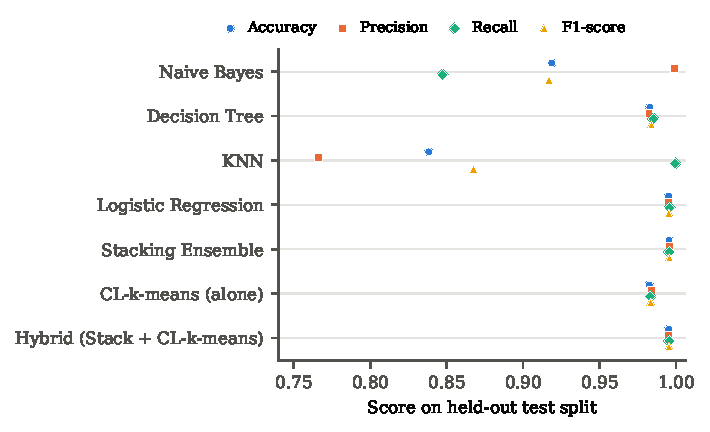
\includegraphics[width=\columnwidth]{fig_metrics}
\caption{Test metrics per model. The axis is zoomed because the dot plot has no baseline.}
\label{fig:metrics}
\end{figure}

With the validation-selected $\tau=\CLKtau$, the hybrid achieves \HybAcc\% accuracy (F1 \HybFone). This is essentially the same as Stage~1: the anomaly layer re-labels \StageTwoFlips{} emails as phishing, of which \StageTwoCorrect{} actually are, while Stage~1 had missed \StageOneMissed. If stage~1 is already at close to its maximum, adding a second unsupervised level gives little improvement. This also fits with HMS-IDS where improvements are also due to unknown attack scenario. Fig.~\ref{fig:cm} shows the confusion matrices.

\begin{figure}[t]
\centering
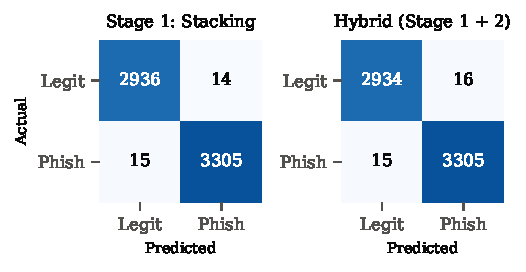
\includegraphics[width=\columnwidth]{fig_confusion}
\caption{Confusion matrices on the test split.}
\label{fig:cm}
\end{figure}

\subsection{Effect of the purity threshold $\tau$}
Table~\ref{tab:tau} shows the security/usability trade-off controlled by $\tau$. Lowering $\tau$ to 0.8 raises in-distribution recall to \TauEightRec{} (\TauEightFN{} missed phishing emails) at the cost of an FPR of \TauEightFPR\%. An organisation that prefers to over-flag could choose this operating point; a personal inbox would keep a strict $\tau$.

\begin{table}[t]
\centering
\caption{Hybrid performance as a function of the purity threshold $\tau$ ($k=\CLKk$)}
\label{tab:tau}
\resizebox{\columnwidth}{!}{\begin{tabular}{ccccccc}
\toprule
 & \multicolumn{3}{c}{In-distribution test} & \multicolumn{3}{c}{CEAS$\rightarrow$Ling}\\
\cmidrule(lr){2-4}\cmidrule(lr){5-7}
$\tau$ & Rec. & FPR & F1 & Rec. & FPR & F1\\
\midrule
Stage 1 only & 0.9955 & 0.0047 & 0.9956 & 0.2626 & 0.0337 & 0.3647\\
0.6 & 0.9988 & 0.0207 & 0.9903 & 0.5252 & 0.4752 & 0.2612\\
0.7 & 0.9988 & 0.0176 & 0.9916 & 0.5230 & 0.4752 & 0.2602\\
0.8 & 0.9988 & 0.0115 & 0.9943 & 0.5098 & 0.4273 & 0.2716\\
0.9 & 0.9964 & 0.0088 & 0.9943 & 0.2954 & 0.1254 & 0.3024\\
0.95 & 0.9955 & 0.0071 & 0.9946 & 0.2691 & 0.1245 & 0.2799\\
0.99 & 0.9955 & 0.0054 & 0.9953 & 0.2691 & 0.1229 & 0.2811\\
1.0 & 0.9955 & 0.0054 & 0.9953 & 0.2670 & 0.1095 & 0.2898\\
\bottomrule
\end{tabular}
}
\end{table}

\subsection{Unseen-corpus (zero-day-style) evaluation}\label{sec:cross}
In order to simulate new phishing attacks, we train our model on a different corpus than it is tested on. We use the same hyper-parameters (Table~\ref{tab:cross}, Fig.~\ref{fig:cross}). The results change sharply. Trained on \XCLNtrain{} CEAS emails and tested on all \XCLNtest{} Ling emails, the stacking ensemble's F1 drops from \StackFone{} to \XCLStackFone, with recall \XCLStackRec{}. Its accuracy of \XCLStackAcc\% is barely above the \LingMajority\% obtained by labelling every Ling email legitimate. The CL-$k$-means layer does not recover the loss (hybrid F1 \XCLHybFone): clusters learned on CEAS do not describe Ling's vocabulary. In the reverse direction, trained on only \XLCNtrain{} Ling emails, the models also degrade (stacking F1 \XLCStackFone). Here the anomaly layer does recover a small number of missed phishing emails (hybrid recall \XLCHybRec{} vs.\ \XLCStackRec{}), and CL-$k$-means on its own (F1 \XLCCLKFone) outperforms the stacking ensemble. This suggests that cluster information can be better transferred than decision boundaries in situations where there is little training data. 

\begin{table}[t]
\centering
\caption{Unseen-corpus results: train on one corpus, test on the other}
\label{tab:cross}
\resizebox{\columnwidth}{!}{\begin{tabular}{lcccc}
\toprule
 & \multicolumn{2}{c}{CEAS $\rightarrow$ Ling} & \multicolumn{2}{c}{Ling $\rightarrow$ CEAS}\\
 & Acc. & F1 & Acc. & F1\\
\midrule
Naive Bayes & 0.8464 & 0.0835 & 0.6592 & 0.7461\\
Decision Tree & 0.7607 & 0.2484 & 0.6734 & 0.6627\\
KNN & 0.1536 & 0.2654 & 0.4781 & 0.1301\\
Logistic Regression & 0.8509 & 0.3983 & 0.8168 & 0.8279\\
Stacking Ensemble & 0.8537 & 0.3647 & 0.7453 & 0.7920\\
CL-k-means alone & 0.4878 & 0.2383 & 0.8153 & 0.8367\\
\textbf{Hybrid (proposed)} & 0.7908 & 0.2898 & 0.7473 & 0.7941\\
\bottomrule
\end{tabular}
}
\end{table}

\begin{figure}[t]
\centering
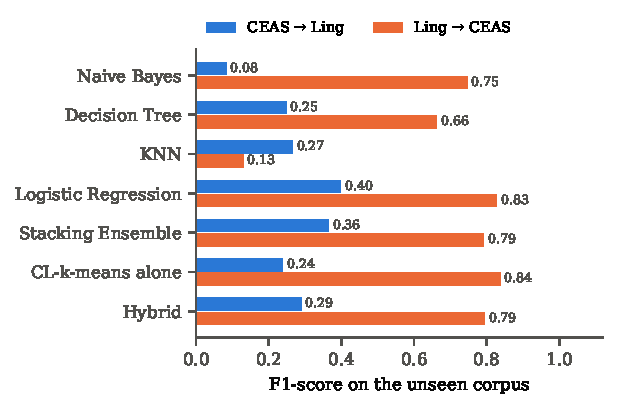
\includegraphics[width=\columnwidth]{fig_cross_corpus}
\caption{F1 on the unseen corpus for both transfer directions.}
\label{fig:cross}
\end{figure}

This gap constitutes the main finding of our study. Learners based on bag-of-words will have learned the vocabulary used in the campaigns in the training set. This means that receiving a high in-distribution score of 99\% tells us nothing about how they would perform on the next campaign. For text-based detectors, a near-perfect in-distribution score should therefore be complemented by a cross-corpus evaluation. This gap also provides motivation for Stage~3. As the LLM does not receive any corpus specific training, the errors it makes are not specific to the vocabulary of the training corpus. Section~\ref{sec:llm} tests whether this holds in practice.

\subsection{LLM stage}\label{sec:llm}
\ifnum\HaveGemini=1
Table~\ref{tab:llm} reports the Gemini (\GemModel) results.
\begin{table}[t]
\centering
\caption{LLM (Gemini) zero-shot results compared with the ensemble on the same emails}
\label{tab:llm}
\resizebox{\columnwidth}{!}{\input{table_gemini}}
\end{table}

\else
Stage~3 is implemented and runs in the extension (Section~\ref{sec:ext}); however, we do not yet quantify this. We plan three experiments. 1) Compare Gemini to the ensemble in terms of zero shot accuracy on a balanced test set of emails. 2) Compare Gemini to the CEAS trained ensemble on the Ling emails (where Stages~1--2 fail). 3) Evaluate the three stage process on the test set, where only uncertain emails are escalated. Scripts and cached responses are available in the released code. Results will be presented in the updated version. Any claims that the LLM closes the generalisation gap remain hypotheses at this point.
\fi

\subsection{Run time}
Fig.~\ref{fig:time} reports training and inference time on a 2-core CPU. Stacking trains in \StackTrainTime{}~s and classifies the whole test split in \StackTestTime{}~s. Most of that time is spent by its KNN member, which compares every email with the whole training set; the other learners take a fraction of a second. This is one of the reasons Stage~3 is called only for uncertain emails.

\begin{figure}[t]
\centering
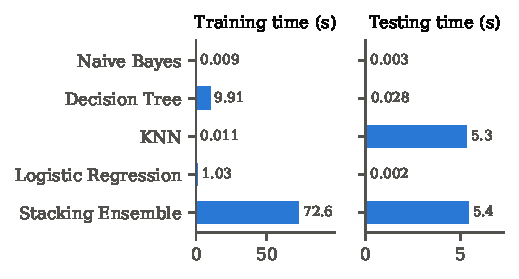
\includegraphics[width=\columnwidth]{fig_time}
\caption{Training and testing time per base learner (test split, 2-core CPU).}
\label{fig:time}
\end{figure}

% =====================================================================
\section{Limitations and Future Work}
Both corpora are quite dated (Ling-Spam was created in 2000, CEAS in 2008). Many of the samples in the 'phishing' class are actually spam samples. This means that the absolute numbers may not reflect current threats. Finally, exact duplicates are removed, meaning that near duplicates can still exist and potentially inflate performance on in-distribution data. The LLM stage inherits prompt-injection risk \cite{greshake2023indirect}, and its verdicts depend on a model version that the provider can change or retire. Future work will add recent phishing corpora (e.g., the other datasets in \cite{champa2023zenodo}), use URL and email-header features, test lightweight local LLMs so that email content stays on the device, and update the clusters as new campaigns appear, as proposed by HMS-IDS.

% =====================================================================
\section{Conclusion}
We adapted the HMS-IDS two-tier architecture of a stacking ensemble followed by a cluster-labelling $k$-means anomaly layer from industrial-IoT intrusion detection to phishing email detection. We extended our algorithm with LLM escalation and implemented it in a Gmail browser extension. The ensemble achieved almost perfect performance in distribution (\StackAcc\% accuracy). Under an unseen-corpus protocol, however, its F1 drops to \XCLStackFone. The unsupervised layer does not help close the gap. This shows that the most important thing when assessing a phishing detection system is to report the gap. To see how well the LLM layer helps close this, we can calculate it.

\section*{Acknowledgment}
We thank Dr. Kumar Saurabh, Bennett University, for his guidance throughout this work.

The browser extension and Gemini prompt build on the open-source CMPE209FinalProject by E.~Pham, T.~Bui and H.~Chen \cite{cmpe209repo}. The datasets were curated by Champa \emph{et al.} \cite{champa2023zenodo}.


\bibliographystyle{IEEEtran}
\bibliography{references}

\end{document}
